%%%%%%%%%%%%%%%%%%%%%%% file template.tex %%%%%%%%%%%%%%%%%%%%%%%%%
%
% This is a general template file for the LaTeX package SVJour3
% for Springer journals.          Springer Heidelberg 2010/09/16
%
% Copy it to a new file with a new name and use it as the basis
% for your article. Delete % signs as needed.
%
% This template includes a few options for different layouts and
% content for various journals. Please consult a previous issue of
% your journal as needed.
%
%%%%%%%%%%%%%%%%%%%%%%%%%%%%%%%%%%%%%%%%%%%%%%%%%%%%%%%%%%%%%%%%%%%
%
% First comes an example EPS file -- just ignore it and
% proceed on the \documentclass line
% your LaTeX will extract the file if required
\begin{filecontents*}{example.eps}
%!PS-Adobe-3.0 EPSF-3.0
%%BoundingBox: 19 19 221 221
%%CreationDate: Mon Sep 29 1997
%%Creator: programmed by hand (JK)
%%EndComments
gsave
newpath
  20 20 moveto
  20 220 lineto
  220 220 lineto
  220 20 lineto
closepath
2 setlinewidth
gsave
  .4 setgray fill
grestore
stroke
grestore
\end{filecontents*}

\RequirePackage{fix-cm}
%
%\documentclass{svjour3}                     % onecolumn (standard format)
\documentclass[smallcondensed,natbib]{svjour3}     % onecolumn (ditto)
%\documentclass[smallextended]{svjour3}       % onecolumn (second format)
%\documentclass[twocolumn]{svjour3}          % twocolumn
%
\smartqed  % flush right qed marks, e.g. at end of proof
%
\usepackage{graphicx}
%
\usepackage{mathptmx}      % use Times fonts if available on your TeX system
%
% insert here the call for the packages your document requires
\usepackage{latexsym}
% etc.
%
% please place your own definitions here and don't use \def but
% \newcommand{}{}
%
\journalname{Climatic Change}
%
\begin{document}

\title{Spatial modelling of rice yield losses in Tanzania due to bacterial leaf blight and leaf blast in a changing climate\thanks{The authors wish to acknowledge J.K. Aunario and M. Noel for their assistance in running models and gathering data used in this study. The authors were funded in part by the Mitigating the Impact of Climate Change On Rice Disease resistance in East Africa (MICCORDEA) project financed by Deutsche Gesellschaft f{\"u}r Internationale Zusammenarbeit (GIZ), by the Consultative Group for International Agricultural Research (CGIAR) Consortium Research Programs (CRP) Climate Change, Agriculture and Food Security (CCAFS) and Global Rice Science Partnership (GRiSP).}}

%\subtitle{Do you have a subtitle?\\ If so, write it here}

\titlerunning{Spatial modelling of rice yield losses in Tanzania in a changing climate}

\author{Confidence Duku\thanks{The first two authors contributed equally to this work and are listed alphabetically.} \and
		Adam H. Sparks \and
		Sander J. Zwart
}

%\authorrunning{Short form of author list} % if too long for running head

\institute{C. Duku \and S. Zwart \at
              Africa Rice Center (AfricaRice), 01 BP 2031, Cotonou, Benin \\
              Tel.: +229-6418-1313 through 1616, Fax: +22-6422-7809\\
              \email{s.zwart@cgiar.org}\\
             \emph{Present address C. Duku: Environmental Systems Analysis Group, Wageningen University, P.O. Box 47, 6700 AA Wageningen, The Netherlands} %  if needed
           \and
           A.H. Sparks \at
              International Rice Research Institute (IRRI), DAPO Box 7777, Metro Manila, 1301, Philippines
}


\date{Received: date / Accepted: date}
% The correct dates will be entered by the editor


\maketitle

\begin{abstract}
Rice is the most rapidly growing staple food in Africa and although rice production is steadily increasing, the consumption is still out-pacing the production. In Tanzania, two important diseases in rice production are leaf blast caused by \textit{Magnaporthe oryzae} and bacterial leaf blight caused by \textit{Xanthomonas oryzae} pv. \textit{oryzae}. The objective of this study was to quantify rice yield losses due to these two important diseases under a changing climate. We found that bacterial leaf blight is predicted to increase causing greater losses than leaf blast in the future, with losses due to leaf blast declining. The results of this study indicate that the effects of climate change on plant disease can not only be expected to be uneven across diseases but also across geographies, as in some geographic areas losses increase but decrease in others for the same disease.
\keywords{EPIRICE \and RICEPEST \and Sub-Saharan Africa \and \textit{Magnaporthe oryzae} \and \textit{Xanthomonas oryzae} pv. \textit{oryzae}
}
% \PACS{PACS code1 \and PACS code2 \and more}
% \subclass{MSC code1 \and MSC code2 \and more}
\end{abstract}

\section{Introduction}
\label{intro}
Rice is the most rapidly growing staple food in Africa and although rice production is steadily increasing, the consumption is still out-pacing the production. For example, by 2009 37 percentof the rice consumed in Africa was imported. To reduce its reliance on imports and dependency on global markets Africa's rice production needs to increase further \citep{Seck2013}. Current average yield levels in Africa range from about 1 t ha\textsuperscript{-1} in upland ecologies to 1.5 to 2 t ha\textsuperscript{-1} in rainfed lowland ecologies with the irrigated lowland ecologies having the highest yields of 3.0 to 4.0 t ha\textsuperscript{-1} \citep{Diagne2013}. Rice yields in African farmers fields are low due to a combination of abiotic and biotic stresses that constrain them. Farmers can significantly reduce the yield gaps with improved field, water and crop management, and weed control \citep{Saito2013}.
    
    Apart from weeds, pests and diseases also are major biotic stresses that can cause significant reductions in rice yields. Two important diseases in rice are leaf blast (LB) caused by \textit{Magnaporthe oryzae} and bacterial leaf blight (BB) caused by \textit{Xanthomonas oryzae} pv. \textit{oryzae} \citep{Verdier2012}. Because infectious plant disease occurs as an interaction of a favorable environment, a susceptible host and a competent pathogen \citep{Madden2007}, weather conditions impact both the occurrence and gravity of plant disease. Climate change is likely to affect plant disease \citep{Anderson2004,Coakley1999,Garrett2006} and several others have expressed interest in changes to plant disease as a result of climate change \citep{Chakraborty2011,Juroszek2011,Luck2011,Pautasso2010,Savary2011,Sutherst2011}. Moreover, intensification of rice production, which was witnessed in Sub-Saharan Africa since the food crisis of 2008 \citep{Saito2013}, may lead to an increased yield loss due to the blast, thus reducing the benefits that were created \citep{Sere2013}. Increases in disease incidence and severity may deter farmers from investing in intensification measures because of risks related to yield losses or even total crop failure. To the authors' knowledge, the impact of climate change on leaf blast and bacterial leaf blight diseases of rice in Africa has not yet been investigated.
    
    Efforts to link plant disease models with a geographic information system (GIS) to assess the impact of plant diseases spatially include maps of the global number of pesticide applications necessary to control potato late blight using contemporary weather data \citep{Hijmans2000}. While a meta-model to generate map estimates of changes in global potato late blight due to climate change has also been developed \citep{Sparks2014}. Savary et al developed EPIRICE, a GIS--linked plant disease severity model capable of simulating several important diseases of rice, including leaf blast and bacterial leaf blight amongst others \citep{Savary2012}. Most recently, \citep{Kim2015} used a modified version of the EPIRICE model to evaluate the potential impacts of climate change on leaf blast and sheath blight in South Korean rice.
    
    The objective of the study was to quantify the impact of climate change as forecasted by the Intergovernmental Panel on Climate Change (IPCC) on rice yield loss as result of BB and LB. To carry out this study, we linked two previously unlinked, existing models, EPIRICE and RICEPEST \citep{Willocquet2000,Willocquet2002}, and we applied them using spatially and temporally downscaled climate change data to generate predictions on changes in plant disease impact due to climate change in Tanzania.
    
    The linkage of EPIRICE with RICEPEST gives two advantages. First, RICEPEST has been used to estimate yield losses due to diseases and other pest injuries in rice in varying production situations with current weather and climate conditions. However, as plant diseases are affected by weather, the linkage with EPIRICE allows us to model the effects of climate change on both the rice crop and on the diseases while using the same weather data inputs. Second, the spatial nature of EPIRICE outputs enabled us to use RICEPEST in a GIS. Until now RICEPEST yield loss estimates have not been linked to a GIS. Linking RICEPEST with a GIS allowed us to map yield losses for the whole country of Tanzania, rather than just point based predictions of yield losses.
    
    This paper will continue with a justification for the study area, followed by descriptions of the EPIRICE and RICEPEST models. We will then elaborate the framework for assessing rice yield losses under climate change that links both models. The procedure for generating daily weather inputs from the downscaled climate scenarios is outlined followed by the choice of production situations. Next the results are presented, followed by a discussion and finally conclusions.
    
\section{Materials and Methods}
\label{m_and_m}
\subsection{The study region}
\label{study_region}
        Rice accounts for five percent of the total value of agricultural production in Tanzania and is the seventh most important agricultural crop with steadily increasing production over the last decade. However, rice yields in Tanzania remain significantly lower than in neighboring countries \citep{Barreiro-Hurle2012}.
    
    Tanzania was chosen as the study region because of its location in sub-Saharan Africa, the probable effects of climate change in the region and rice is planted widely across the country  (Table 1) \citep{Rowhani2011}. The bulk of the rice crop is grown from December until June of the following year during the rainy season. 
    
    According to the International Panel on Climate Change (IPCC), East Africa and especially the Great Lakes Region are among the more vulnerable regions in Africa to climate change, where the trend is towards increasing temperatures and declining rainfall according to General Circulation Model outputs \citep{Boko2007}. Temperatures are predicted to increase 2$^{\circ}$C by 2050, which in turn are predicted to negatively affect rice yields \citep{Rowhani2011}.
    
    \subsection{Model descriptions}
    \label{model_desc}
    \subsubsection{The EPIRICE model} \label{EPIRICE}
    EPIRICE \citep{Savary2012} is a SEIR (susceptible-exposed-infectious-removed) model \citep{Kermack1927,Madden2006} implemented in R \citep{R2014} that simulates potential spatial epidemics of rice diseases including BB and LB. The model considers a 1m\textsuperscript{2} area of rice, which is the same area that RICEPEST considers, with maximum host susceptibility to the given disease. Model inputs are date of crop establishment and daily time-step weather data; precipitation, maximum and minimum temperature, and relative humidity. The model as originally implemented produces a single aggregated output, a map, at the end of a growing season of a measure called Area Under Disease Progress Curve (AUDPC) \citep{Madden2007}. However, for this study, daily disease severity expressed as a percentage was generated for use in the RICEPEST model, which we discuss further in section \ref{RICEPEST}. As the only modification made to the model was the expression of daily disease severity, we  would refer the reader to \citep{Savary2012} for further information on the model structure and function.
    
    \subsubsection{The RICEPEST model}\label{RICEPEST}
    The RICEPEST model \citep{Willocquet2000,Willocquet2002} simulates rice yield losses due to several yield-reducing factors under a range of specific production situations with simulated diseases including BB and LB. The model runs on a daily time-step with simulation starting 14 days after crop establishment for both transplanted and direct seeded rice. The model incorporates two sub-models, the first sub-model simulates the dynamics of the rice crop biomass and the second sub-model simulates the dynamics of the tiller population. The biomass sub-model accounts for the daily accumulation and partitioning of assimilates towards roots, leaves, stems, and panicles. For this study, because the damage mechanisms of the diseases of interest (BB and LB) are simulated only in the biomass sub-model, the tiller sub-model was not considered.
    
    bacterial leaf blight and LB cause lesions on the leaf blades. These lesions decrease the green leaf area index (LAI), reducing the photosynthetic capacity of the plant. RICEPEST reduces the rate of growth (RG) (Formula \ref{RG}) by reducing the LAI (Formula \ref{LAI}) by applying a damage function (Formula \ref{BBDM}) or (\ref{LBDM}) where SLA is the specific leaf area; LEAFW is the leaf dry weight; RUE is radiation use efficiency; RAD is daily solar radiation; k is coefficient of light extinction and is defined as the proportion of light intercepted by the crop \citep{Willocquet2000}, set to 0.6 \citep{Willocquet2002}.
    \begin{equation}
    RG_t = RUE_t \times RAD_t \times (1- exp(- k \times LAI_t))
    \label{RG}
    \end{equation}
    
    \begin{equation}
    LAI_t = SLA_t \times LEAFW_t
    \label{LAI}
    \end{equation}
    The damage functions that calculate the reduction factors, BBDM (Formula \ref{BBDM}) and LBDM (Formula \ref{LBDM}) are the percent of leaf area covered by BB and LB respectively \citep{Willocquet2002}, which were generated as raster files for use in this version of RICEPEST using the EPIRICE model as described in the previous section, \ref{EPIRICE}. 
    \begin{equation}
    (1-(BBDM_t /100)
    \label{BBDM}
    \end{equation}
    
    \begin{equation}
    (1-(LBDM_t /100))
    \label{LBDM}
    \end{equation}
    Thus, the complete LAI formula with the damage function for BB reducing the photosynthetic area of the leaf becomes
     \begin{equation}
    LAI_t = SLA_t \times LEAFW_t \times (1-(BBDM_t / 100)).
    \label{LAIBBDM}
    \end{equation}
    
    \subsubsection{Model coupling}
    \label{model_coupling}
    To facilitate coupling of EPIRICE to RICEPEST, a temporal disaggregation function was incorporated into the EPIRICE model. With this function, the modified EPIRICE model produced daily, spatially representative and non-cumulative percentage disease severity data as outputs instead of the single cumulated output, AUDPC. The time-series of daily percentage disease severity data for BB and LB produced by the modified EPIRICE model were then used as inputs for RICEPEST. Both models were linked to a geographic information system (GIS). EPIRICE is implemented in the R language using the following packages, cropsim \citep{Hijmans2009}, oldweather \citep{Hijmans2009}, raster \citep{Hijmans2014}, rgdal \citep{Bivand2014}, and RODBC \citep{Ripley2013}, while this version of RICEPEST is implemented in Python language \citep{python}, using the ArcPy package, as a script in the ArcGIS platform \citep{ESRI2011}. A loose coupling approach was adopted due to the different implementation environments. This approach provided flexibility in data handling and data interoperability (Figure \ref{Fig1}).
        
    \subsection{Growing seasons and areas}
    \label{growings_seasons}
    The major planting window in Tanzania for most rain-fed ecologies in Tanzania, according to the FAO Crop Calendar database \citep{FAOCropCalendar}, was October to December, with the largest area of Tanzania being planted in late November. Because the original climate data were monthly, not daily and needed to be temporally downscaled, a planting window of late November to early December was selected and ArcGIS was used to create a spatial dataset of areas with this planting window. Annual harvested rain-fed rice growing areas for Tanzania with values representing the proportion of harvested areas (in hectares) within each pixel (10,000 ha) was also obtained from MIRCA2000 \citep{Portmann2010}. To select the major rice growing areas in Tanzania during this planting window, a simple raster overlay analysis was performed in ArcGIS.
    
    \subsection{Weather Data Generation}
    \label{weather_data}
    For this study, the General Circulation Model (GCM), Commonwealth Scientific and Industrial Research Organization mark 3 (CSIRO-MK3) was selected. Downscaled outputs from this GCM based on three future climate scenarios A1B, A2 and B1 as reported in the Special Report on Emission Scenarios (SRES) of the IPCC Fourth Assessment Report, for two time slices 2030s (2021-2040) and 2050s (2041-2060) were obtained. A2 is a high greenhouse gas emission scenario; A1B, a medium-emission scenario; and B1, a low-emissions scenario. The selection of the GCM and the emission scenarios were based on the availability of complete downscaled climate data to run both models. Monthly projected precipitation, minimum and maximum temperature, solar radiation and wet day frequency outputs of this GCM, spatially downscaled to approximately 10km by 10km grid resolution using a pattern scaling approach were obtained from International Center for Tropical Agriculture's (CIAT) CGIAR Research Program on Climate Change, Agriculture and Food Security (CCAFS) Geoportal (http://www.ccafs-climate.org) \citep{Jones2009}. However, relative humidity outputs of this GCM were obtained directly from the CMIP3 dataset and spatially downscaled to 10km by 10km using statistical downscaling delta technique. Observed climate data for the period 2000s (1991-2010) was obtained from the same source and used as the baseline for this study. A parametric stochastic weather generator, MODAWEC \citep{Liu2009}, which requires only monthly data (as outlined in \citep{Geng1986} and MODAWEC) was used to generate daily precipitation, maximum and minimum temperature datasets corresponding to future scenarios. This was essential in producing daily minimum and maximum temperature data that correlate with precipitation. A linear interpolation technique was, however, used in generating daily relative humidity and solar radiation from monthly data. The daily weather data generated were used as inputs in both EPIRICE and RICEPEST models.
    
    \subsection{Production situation}
    \label{production_situation}
    Rice production situations have been found to directly affect the intensity of rice yield reduction for a given injury profile. That is, the farmers' practices play a large part in determining what the diseases and injuries will occur \citep{Savary2000}. For this study, production situation is defined as the combination of socioeconomic, environmental and biophysical factors excluding pests that define the attainable yield. Temperature and solar radiation were excluded from this definition because they remain unchanged across all the possible production situations in the study area. Due to lack of reliable information about the spatial arrangement of production situations in the study area, the production situation was assumed to be homogeneous based on the most common production situation, lowland rainfed rice \citep{Diagne2013} (Table 1). We created a production situation based on PS3 from \citep{Willocquet2004}. A short duration cultivar, transplanted with poor water management and medium water stress and 90kg/ha nitrogen fertilization with a modified STEMP from PS4. This modification was due to differences in temperature between Tanzania and Faizabad, Uttar Pradesh, India, the source of the original weather data for simulations in RICEPEST.
    
    \subsection{Spatial modelling of yield loss}
    \label{modelling_yield_loss}
    Simulation runs of EPIRICE and RICEPEST were made separately at a spatial resolution of 10km by 10km for the growing season December to March for current climate conditions, the 2000 time slice, and for each of the three emission scenarios, A1B, A2 and B1, for both the 2030 and the 2050 time slices. These data only included precipitation and temperature changes. The effects of changes CO$_{2}$ levels on the plant host or pathogens were not considered as a part of this study.
    
    To map and quantify the spatial distribution of rice yield loss as a result of the two diseases under current and future climate conditions, the RICEPEST model was run using daily temperature and solar radiation data and daily disease severity outputs from the EPIRICE model within the ArcGIS environment using the aforementioned Python tool in ArcGIS. Simulation runs were first made without the injury profiles to obtain the attainable yield. Maintaining the same weather data and production situation parameter values, simulation runs were then made with the treatment of injury profiles to obtain the actual yield in the presence of the two diseases separately (Figure \ref{Fig1}). Yield loss was then modelled as the difference between attainable yield and actual yield for both BB and LB damaged crops respectively.
    
    \section{Results and discussion}
    \label{results_and_discussion}
    
    \subsection{Changes in temperature}
    \label{temperature_changes}
    The average base temperature for Tanzania used in this data was 22.69 $^{\circ}$C, with all succeeding time slices increasing in average temperature (Table \ref{tab:change}). The average increase in future time slices due to climate change was 1.17 $^{\circ}$C (Table \ref{tab:change}).
    
    
    % For tables use
\begin{table}
\caption{Average temperature and change in temperatures  for Tanzania from the base 2000 time slice for IPCC A1B, A2 and B1 scenarios for 2030 and 2050 time slices for the months of November through February. The 2000 time slice represents 1991-2010, 2030 time slice represents 2021-2040, the 2050 time slices represents 2041-2060.}
\label{tab:change}       % Give a unique label
% For LaTeX tables use
    \begin{tabular}{@{}lcc@{}}
\hline\noalign{\smallskip}
Scenario and Time Slice      & Average Temperature ($^{\circ}$C) & Change in Temperature ($^{\circ}$C)  \\
\noalign{\smallskip}\hline\noalign{\smallskip}
	Base 2000 	& 22.69                       & -                                   \\
    A2 2030  	& 23.88                       & 1.19                                \\
    A2 2050  	& 24.38                       & 1.68                                \\
    A1B 2030   	& 23.73                       & 1.04                                \\
    A1B 2050   	& 23.95                       & 1.25                                \\
    B1 2030   	& 23.48                       & 0.79                                \\
    B1 2050   	& 23.73                       & 1.04                                \\ 
\noalign{\smallskip}\hline
\end{tabular}
\end{table}  

\subsection{Potential disease epidemics (EPIRICE model output)}
\label{potential_epidemics}
    Predicted leaf blast epidemics were not severefor the entire country. Severity of the disease was predicted to be less than 2.5 percent across Tanzania for all time slices and emission scenarios (Figure \ref{Fig2}). Disease peaks halfway through the season, which is characteristic of this disease that tends to occur during vegetative growth stages before the crop reaches reproductive stages and final maturity.
    
    bacterial leaf blight epidemics exhibited normal progress curves for the disease with a much greater severity in all time slices than that of LB. Under all time slices and scenarios the predicted epidemic started rapidly increasing around day 50 and increased up until day 100, when it began decreasing at crop maturity (Figure \ref{Fig3}), which is normal for this disease. The three different emission scenarios resulted in differing AUDPC responses for bacterial leaf blight across the time slices. The A2 scenario resulting in the highest predicted disease levels, the B1 scenario was the lowest.
        
    \subsection{Predicted yields and yield losses (RICEPEST model output)}
    \label{predicted_yields}
    \subsubsection{Attainable yields}
    \label{attainable_yields}
    RICEPEST predicted the mean attainable yields under the current conditions, in the absence of yield reducing factors, to be 3.88 t ha\textsuperscript{-1} for the current rice growing areas of Tanzania for the base climate (Figure \ref{Fig4}). Future conditions were all predicted to have higher mean attainable yields. All simulated time-slices exhibited a minimal amount of values that were reported as zero t ha\textsuperscript{-1}.
    
    \subsubsection{Yield losses due to leaf blast}
    \label{lb_yield_losses}
    Differences due to leaf blast between all time slices and scenarios were negligible (Figure \ref{Fig5}). The base had the highest average yield loss values due to leaf blast, 0.12 t ha\textsuperscript{-1}. However, the B1 2050 scenario exhibited the lowest average yield losses of any scenario and time slice combination, but the highest values at 0.13 t ha\textsuperscript{-1} lost.
       
    \subsubsection{Yield losses due to bacterial leaf blight}
    \label{bb_yield_losses}
    bacterial leaf blight was predicted to cause much greater losses than leaf blast (Figure \ref{Fig6}). The overall trend in losses due to bacterial leaf blight was up for all three climate scenarios, from the Base 2000. The A2 2050 and AB 2050 scenario and time slices had the highest average predicted values with 0.73 t ha\textsuperscript{-1} lost due to bacterial leaf blight. The A2 2030 scenario and time slice registered the single highest losses, 1.44 t ha\textsuperscript{-1}.
        
    \section{Conclusions and discussions}
    \label{conclusions}
    The loose coupling approach that we adopted for this research has proven to be useful. It allows for us to examine patterns and trends that previously we were unable to easily examine. This approach should prove useful for further work where spatial modelling of rice yield loss is desired for both current conditions and future predictions.
    
    Some initial difficulties in selecting the proper production situation for an area outside the original application domain of the model were experienced. Because the original PS3 was based in Faizabad, Uttar Pradesh, India, the temperatures and duration of the rice were too long to be consistent with Tanzania. Because of this, we elected to modify the model using currently available information in the model itself based on our determinations of what best matched the situation on the ground. The results of the modified RICEPEST model seem to better represent possible scenarios than the original unmodified model was able to.
    
    The RICEPEST model is a simple empirical crop growth model that does not account for CO$_2$ concentration changes and increases yield as temperature increases, though the temperature to maturity is reached sooner, which reduces net biomass accumulation. A next logical step for climate change studies could be to link EPIRICE output with a more advanced model such as ORYZA \citep{Oryza}, although such a linkage will be more difficult due to the added complexity of the ORYZA model.
    
    Despite the predictions of climate change to reduce rice crop yields, this study predicted that the attainable yield would increase with an increase in temperatures. Since the average temperatures were below 24 $^{\circ}$C, it is likely that this would be the case as temperatures below 20 $^{\circ}$C can cause yield losses, so the increased temperatures are more optimal for tropical rice \citep{Yoshida}.
            
    \citet{Thornton2009} found that climate change effects are likely to be unequal across East Africa when they examined maize and bean crops. Localised adaptations to climate change will be necessary. This seems to be the case when examining the maps of change in yield losses due to BB (Figure \ref{Fig7}). Some areas appear to lose more than a half ton per hectare to BB than they previously have, while others appear to actually lose less to BB, gaining 0.75 t ha\textsuperscript{-1} potential yield due to the reduction in the severity of BB.
    
    The results of this study indicate that the effects of climate change on plant disease can be expected to be uneven as the environment becomes less favourable for some diseases such as LB, it becomes more favorable for others like BB. One thing that the results fail to capture is the variation in weather. Because this exercise is based on time-slice averages, what is captured here is the most likely to occur in a given year based on the climate. Weather patterns have great influence on plant diseases. However, these results should be instructive for breeders and policy makers. We should not ignore leaf blast, however these results indicate that in the future bacterial leaf blight will be more of an issue for rice growers in Tanzania than leaf blast. This information can be useful for breeders and policy makers so breeding efforts for resistance and other mitigation methods can be put into place with this outcome in mind.
    
\section{Software, data and supplementary file availability}
\label{software_and_data_availability}
All code used for analysis and data used in this dataset are available from figshare,\\ http://figshare.com/articles/MICORDEA/1408501, and can also be cloned from GitHub,\\https://github.com/adamhsparks/MICORDEA. A Stella language version of the original, complete version of the RICEPEST model by the original authors, L. Willocquet and S. Savary, is available for download from The American Phytopathological Society Education Center,\\
https://www.apsnet.org/edcenter/advanced/topics/BotanicalEpidemiology/Pages/default.aspx.

KML files of the change in yield losses due to bacterial leaf blight (Figure 7) and attainable yields (Figure 4) are also available in the figshare data and GitHub repository in the ``KML'' folder for further exploration and the ability to interactively explore the changes across time-slices using GoogleEarth.

\section{Author attributions}
\begin{itemize}
\item Inputs preparation (CD, AS)
\item Model coupling and processing (CD, AS)
\item Data analysis (CD, AS, SZ)
\item Manuscript preparation (CD, AS, SZ)
\end{itemize}

% BibTeX users please use one of
\bibliographystyle{spbasic}      % basic style, author-year citations
%\bibliographystyle{spmpsci}      % mathematics and physical sciences
%\bibliographystyle{spphys}       % APS-like style for physics
\bibliography{MICORDEA_References}   % name your BibTeX data base

\newpage
     \begin{figure}
     
      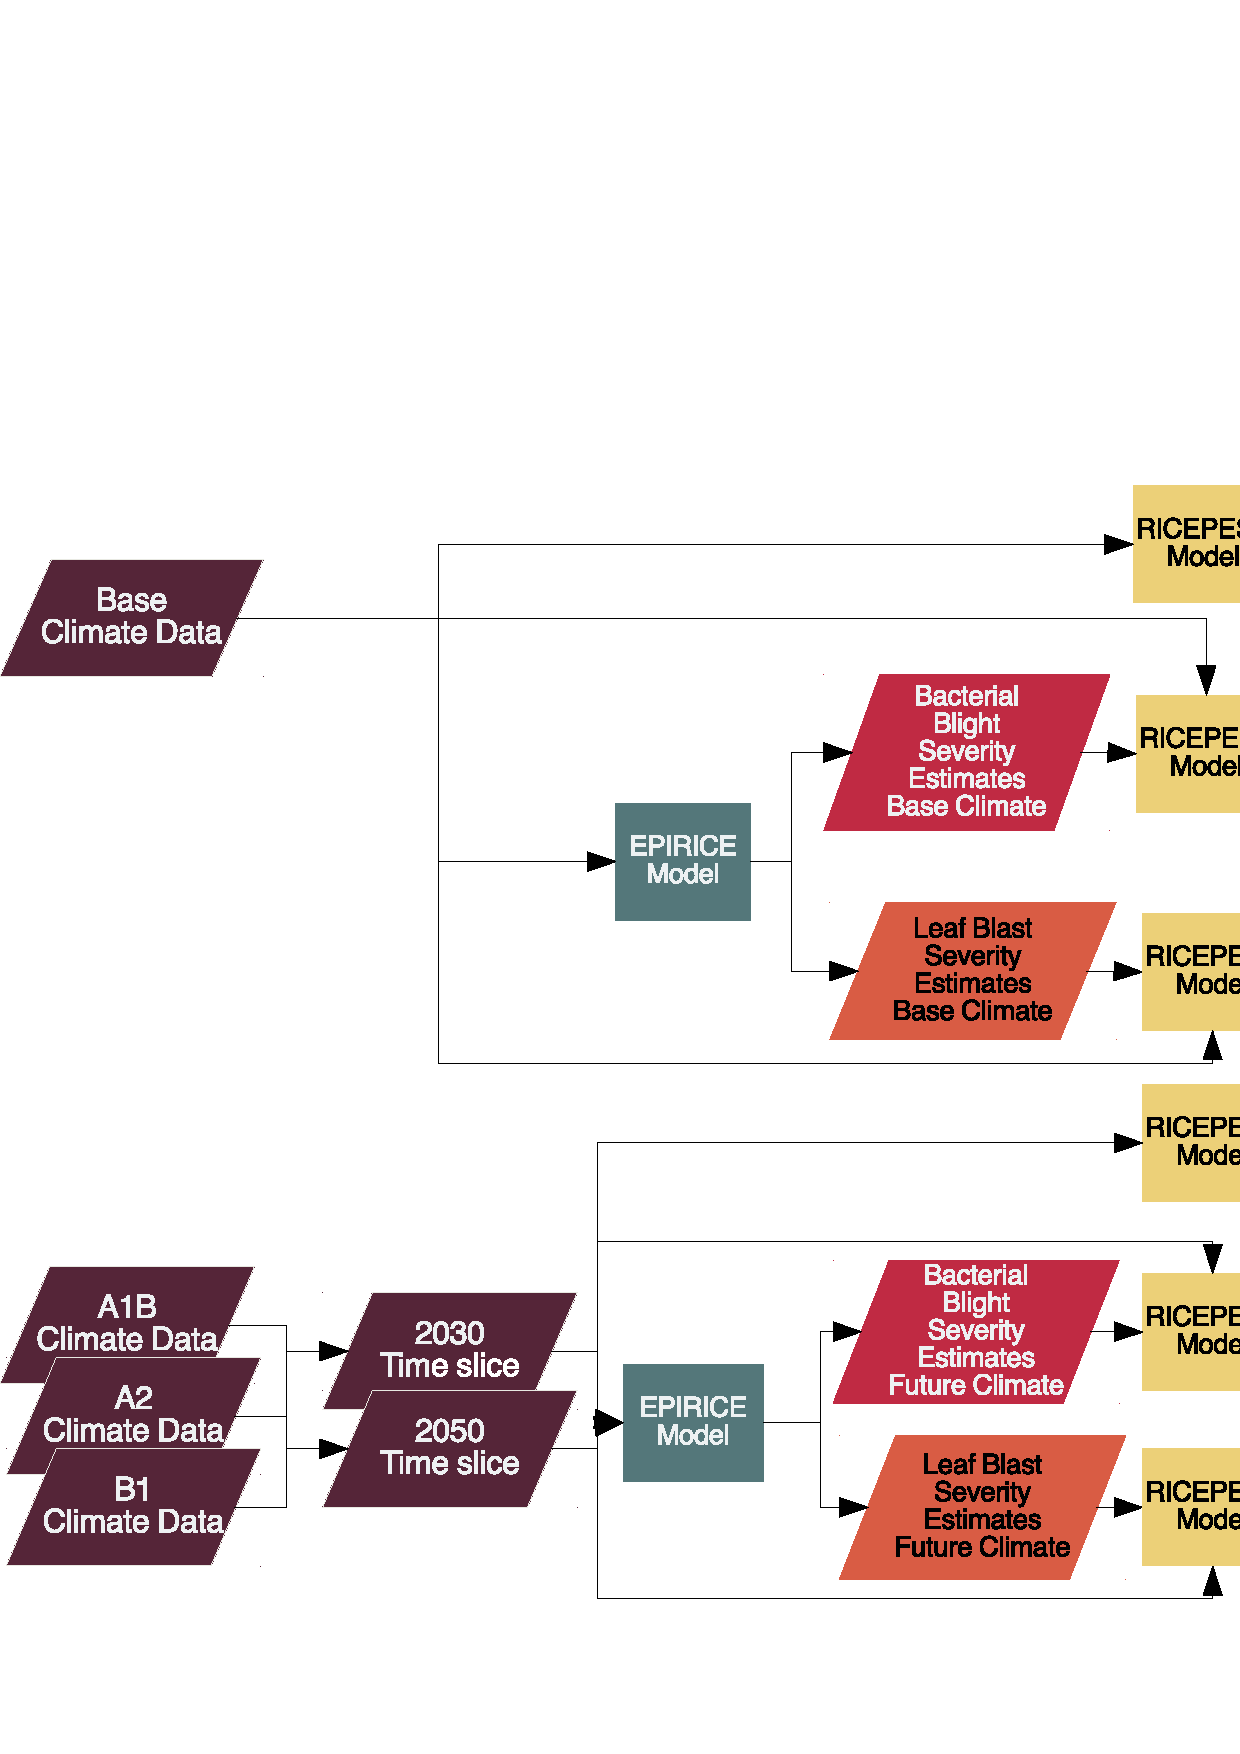
\includegraphics[width = 174mm]{figures/Fig1}
      \caption{Flowchart illustrating the loose coupling between EPIRICE, used to simulate unmanaged disease epidemics as affected by weather conditions, and RICEPEST, used to estimate yield losses due to leaf blast and bacterial leaf blight severity. Three time slices, 2000, 2030 and 2050 were examined for four climate scenarios, current or base, IPCC A1B, IPCC A2 and IPCC B1.}
      \label{Fig1}
    \end{figure} 

    % Leaf blast progress curves
    \begin{figure}
      
\includegraphics[width = 84mm]{figures/Fig2}
      \caption{Leaf blast disease severity curves as predicted by the EPIRICE model averaged for Tanzania.}
        \label{Fig2}
    \end{figure}
    
        % bacterial leaf blight progress curves
    \begin{figure}
      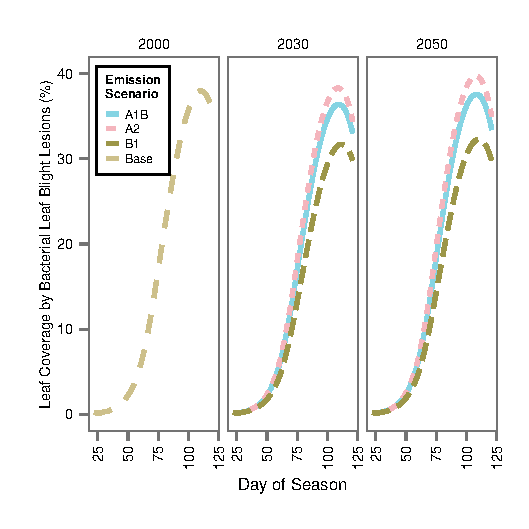
\includegraphics[width = 84mm]{figures/Fig3}
      \caption{Bacterial leaf blight disease severity curves as predicted by the EPIRICE model using observed and future, modelled weather data for three climate change scenarios, A1B; A2 and B1 and three time slices, 2010; 2030 and 2050.}
        \label{Fig3}
    \end{figure}
    
        % Attainable yield loss violin plots
    \begin{figure}
      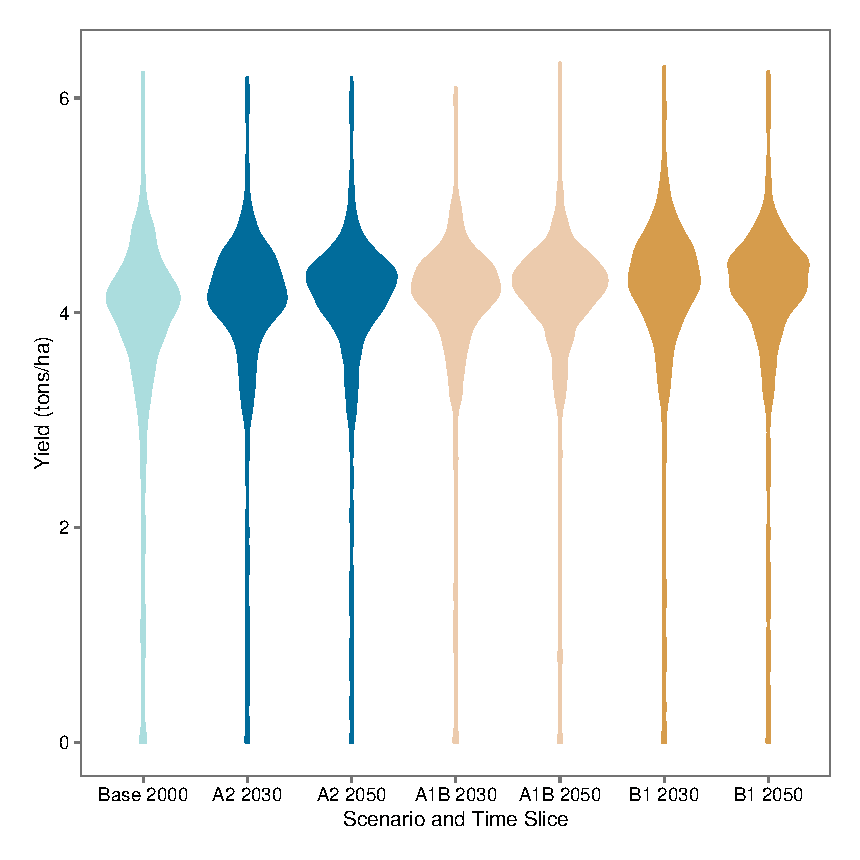
\includegraphics[width = 84mm]{figures/Fig4}
      \caption{RICEPEST predicted attainable yield (i.e., the yield in the absence of yield reducing factors) in t ha\textsuperscript{-1} for all time slices and emission scenarios.}
      \label{Fig4}
    \end{figure}

    % Leaf blast yield loss violin plots
    \begin{figure}
      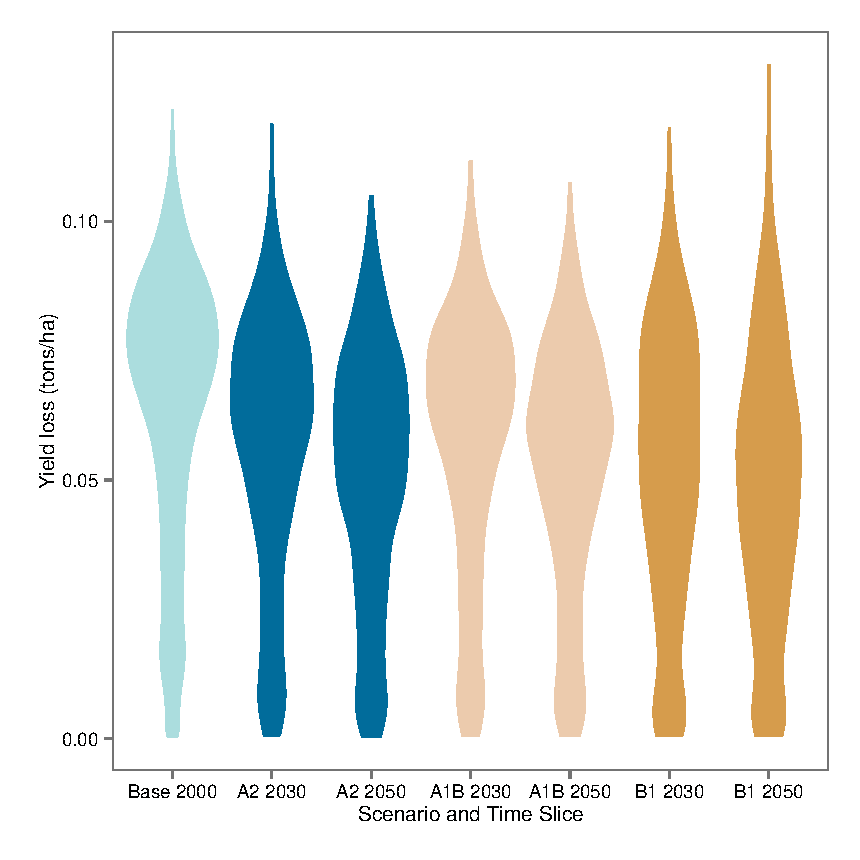
\includegraphics[width = 84mm]{Figures/Fig5}
      \caption{Yield losses in t ha\textsuperscript{-1} due to leaf blast as predicted by the EPIRICE and RICEPEST model three time slices and three IPCC climate emission scenarios.}
      \label{Fig5}
    \end{figure}

    % bacterial leaf blight yield loss violin plots
    \begin{figure}
      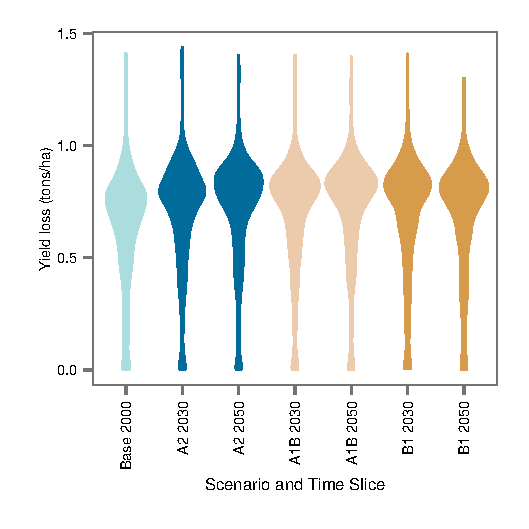
\includegraphics[width = 84mm]{Figures/Fig6}
      \caption{Yield losses in t ha\textsuperscript{-1} due to bacterial leaf blight as predicted by the EPIRICE and RICEPEST model three time slices and three IPCC climate emission scenarios.}
      \label{Fig6}
    \end{figure}
    
    % Bacterial leaf blight yield loss change maps
    
    \begin{figure}
      \includegraphics[width = 174mm]{Figures/Fig7}
      \caption{Changes in yield losses due to bacterial leaf blight disease expressed as t ha\textsuperscript{-1} for all time slices and emission scenarios as predicted using a combination of EPIRICE and RICEPEST models. }
      \label{Fig7}
    \end{figure}

\end{document}


% end of file template.tex

